\documentclass[11pt]{article}
\usepackage[T1]{fontenc}
\usepackage[utf8]{inputenc}
\usepackage{lmodern}
\usepackage[a4paper,margin=29mm]{geometry}
\usepackage{amsmath,amssymb,amsthm,mathtools}
\usepackage{microtype}
\usepackage[numbers,sort&compress]{natbib}
\usepackage{tikz}
\usetikzlibrary{arrows.meta,positioning,calc}
\usepackage{flafter}
\usepackage{url}
\def\UrlBreaks{\do\/\do-\do.\do_}
\Urlmuskip=0mu plus 1mu
\usepackage[colorlinks=true,linkcolor=blue!45!black,citecolor=blue!45!black,urlcolor=blue!45!black]{hyperref}
\hypersetup{pdftitle={Failure of rational injectivity for maximal coarse assembly},pdfauthor={OpenAI},pdfsubject={Coarse geometry, maximal Roe algebras, and integral K-homology}}
\pdfinfoomitdate=1
\pdftrailerid{}
\pdfsuppressptexinfo=15
\numberwithin{equation}{section}
\newtheorem{theorem}{Theorem}[section]
\newtheorem{proposition}[theorem]{Proposition}
\newtheorem{lemma}[theorem]{Lemma}
\newtheorem{corollary}[theorem]{Corollary}
\theoremstyle{definition}
\newtheorem{definition}[theorem]{Definition}
\newtheorem{remark}[theorem]{Remark}
\newcommand{\C}{\mathbb C}
\newcommand{\Z}{\mathbb Z}
\newcommand{\N}{\mathbb N}
\newcommand{\Q}{\mathbb Q}
\newcommand{\R}{\mathbb R}
\newcommand{\K}{\mathcal K}
\DeclareMathOperator{\KK}{KK}
\DeclareMathOperator{\KX}{KX}
\DeclareMathOperator{\id}{id}
\DeclareMathOperator{\prop}{prop}
\DeclareMathOperator{\supp}{supp}
\DeclareMathOperator{\Ad}{Ad}
\DeclareMathOperator{\SL}{SL}
\emergencystretch=1em

\title{Failure of rational injectivity for maximal coarse assembly}
\author{OpenAI}
\date{October 5, 2026}
\begin{document}
\maketitle
\begin{abstract}
We construct a uniformly discrete bounded-geometry space whose maximal coarse
assembly map has an infinite-order element in its kernel. The space is a coarse
disjoint union of finite connected graphs of uniformly bounded degree, so
maximal coarse assembly need not be rationally injective even for such graph
unions.
\end{abstract}
\section{Introduction}\label{sec:introduction}

Coarse assembly relates the topology visible at bounded scales in a metric
space to the indices of operators controlled by its large-scale geometry.
Its rational injectivity asks whether a non-torsion topological class can
have zero coarse index. We prove that this can occur even when the analytic
target is the maximal Roe algebra and the space is a coarse disjoint union
of finite graphs of bounded degree.

Let $Z$ be a uniformly discrete proper metric space of bounded geometry;
thus every ball of a fixed radius contains a uniformly bounded number of
points. Write $P_r(Z)$ for the Rips complex whose simplices are the finite
subsets of diameter at most $r$, and set
\[
 \KX_q(Z)=\varinjlim_{r\to\infty}\KK_q(C_0(P_r(Z)),\C).
\]
All K-theory and K-homology in this article are complex. On the ample module
$H_Z=\ell^2(Z)\otimes\ell^2(\N)$, let $\C[Z]$ be the algebra of bounded,
locally compact, finite-propagation operators. Local compactness means that
$aT$ and $Ta$ are compact for every $a\in C_0(Z)$, and finite propagation
means that $T_{xy}=0$ whenever $d(x,y)$ exceeds some fixed bound. In
particular, the compact matrix entries of $T$ need not satisfy a uniform
rank bound. The universal C*-completion is the \emph{maximal Roe algebra}
$C^*_{\max}(Z)$. The canonical maximal coarse assembly map is
\[
 \mu_Z^{\max}:\KX_q(Z)\longrightarrow K_q(C^*_{\max}(Z)).
\]
We recall the needed norm estimates and the index construction in
Section~\ref{sec:maximal-index}.

A \emph{coarse disjoint union} of finite graphs is a metric on their disjoint
union which restricts to the graph path metric on each component and for
which only finitely many pairs of distinct components are within any fixed
distance. We take such metrics to be uniformly discrete.

\begin{theorem}\label{thm:main}
There exist finite connected graphs $(X_j)_{j\geq1}$ with a common finite
bound on vertex degree, a coarse disjoint union $X=\bigsqcup_{j\geq1}X_j$,
and an infinite-order class $\alpha\in\KX_1(X)$ such that
\[
 \mu_X^{\max}(\alpha)=0.
\]
Consequently, $\mu_X^{\max}\otimes\Q$ is not injective.
\end{theorem}

The theorem strengthens the reduced coarse-assembly result proved in the
companion paper~\cite{OpenAICoarseNovikov2026}.
If $C^*(X)$ denotes the operator-norm
closure of $\C[X]$, the canonical quotient
$C^*_{\max}(X)\to C^*(X)$ carries the maximal index to the reduced index.
Our class $\alpha$ therefore also lies in the reduced assembly kernel. The stronger
conclusion requires a proof in the universal norm: vanishing of a reduced
index alone does not imply vanishing of its maximal lift.

\subsection{Context and prior work}

Roe developed coarse cohomology and coarse index theory as tools for
large-scale geometry and index-theoretic questions on noncompact manifolds
\cite{Roe93}. Higson and Roe formulated and studied the coarse Baum--Connes
conjecture in this framework \cite{HR95}. The connection with Novikov-type
questions is that injectivity retains the topological information carried
by higher indices. The present theorem concerns the non-equivariant coarse
assembly map displayed above.

Several fundamental positive results relate assembly to geometric control.
Yu proved coarse assembly isomorphism for bounded-geometry spaces of finite
asymptotic dimension \cite[Theorem~7.1]{Yu98} and established the coarse
Baum--Connes conjecture for
bounded-geometry spaces admitting a uniform embedding into Hilbert space
\cite{Yu00}. Skandalis, Tu, and Yu developed the coarse-groupoid approach
and its relation to these embedding methods \cite{STY02}. These results
explain the importance of geometric hypotheses when seeking injectivity or
isomorphism theorems.

Earlier failures of injectivity also show why bounded geometry and the
domain of assembly matter. Yu constructed a coarse-assembly kernel class
for a space without bounded geometry \cite[Section~8, Proposition~8.1]{Yu98}.
Dranishnikov, Ferry, and Weinberger constructed integral index-kernel
examples with locally finite K-homology as domain; their kernel classes
disappear under coarsening \cite[Section~6, Remark~6.2]{DFW03}.
Here the class belongs to the actual Rips colimit for a bounded-geometry
graph union and remains nonzero after rationalization.

Finite quotients and expanding graphs also exposed limitations of general
assembly assertions. Higson, Lafforgue, and Skandalis constructed
counterexamples in group and groupoid settings and proved reduced coarse
nonsurjectivity for certain unions of congruence Cayley graphs
\cite[Section~6]{HLS02}. Nonsurjectivity is a different obstruction from
the kernel in Theorem~\ref{thm:main}. Their separate Hausdorff-groupoid
kernel construction combines an odd Bott class with a Kazhdan projection:
a nonzero full-assembly image becomes zero after reduction
\cite[Section~5]{HLS02}. This is a methodological predecessor, but its
behavior also makes it essential to distinguish the two analytic targets.

The maximal Roe algebra and its assembly map were developed in work of
Gong, Wang, and Yu \cite{GWY08} and Oyono-Oyono and Yu \cite{OOY09}; the
latter analyzed maximal assembly for specific families of expanders arising
from finite group quotients. Willett and Yu further studied higher indices
for expanding and large-girth graph families \cite{WY12}.
\v{S}pakula and Willett proved that the maximal-to-reduced comparison
induces a K-theory isomorphism for spaces admitting a coarse embedding into
Hilbert space \cite{SW13}. Chen, Wang, and Yu proved the maximal coarse
Baum--Connes conjecture under the more general hypothesis of a fibred
coarse embedding into Hilbert space \cite{CWY13}. More recent injectivity
results concern finite-group extensions whose kernel and quotient families
admit such fibred embeddings \cite{DGWY25}; maximal isomorphism results also
hold for coarse fibrations with uniformly property-A fibers, a
fibred-coarsely-embeddable base, and uniform coarse equivalences between
fibers and preimages of fixed-radius balls \cite{GWZ25}. Finite fibers alone do not
supply these uniform hypotheses. Theorem~\ref{thm:main}
shows that rational injectivity cannot hold for all bounded-geometry graph
unions without further assumptions.

Our analytic tools belong to this established maximal-index framework.
We give the norm and functoriality arguments needed here, with particular
attention to the points where the universal and operator norms must be
distinguished; see also \cite{OOY09,SW13,SS21}. Kazhdan's property~(T)
\cite{Kazhdan67,BHV08} supplies averaging in the full group C*-algebra.
The topological part uses integral line-bundle classification, the
K-theory of projective spaces, and the standard K-homology pairing
\cite{Atiyah67,Blackadar98,HigsonRoe00}.

\subsection{The construction and the proof}

The base graphs are three-dimensional discrete tori $B_j$ whose side
lengths tend to infinity. Over each $B_j$ we place a finite quotient of
$\SL_3(\Z)$, obtaining a graph $Y_j$ with Cayley edges inside the fibers.
Transport around the first two base circles is given by commuting elements
of that quotient. These elements cease to commute at a higher congruence
level. The graph $X_j$ joins two copies of $B_j$ through $Y_j$: its middle
has a long product collar, and toward either end the fiber quotients are
reduced one level at a time until they become trivial. This keeps all
vertex degrees bounded. Section~\ref{sec:geometry} gives the construction.

Write $B=\bigsqcup_jB_j$, $Y=\bigsqcup_jY_j$, and let
\[
 f:Y\longrightarrow B,\qquad i_\pm:B\longrightarrow X
\]
be the middle projection and the two end inclusions. A torus K-homology
class on each component defines a single class $\beta\in\KX_1(B)$.
The class of interest is
\[
 \alpha=(i_+)_*\beta-(i_-)_*\beta.
\]
Its persistence and its zero index come from different features of the
middle projection.

For persistence, take a line bundle $\mathcal L$ on each continuous base
torus, with first Chern class the product of the first two circle classes.
Its reduced K-theory class, multiplied by the third circle's odd class,
pairs to one with the chosen K-homology class. At every fixed Rips scale,
the lifted commutator calculation shows that the pullback of $\mathcal L$
to the middle admits a $2^j$-th root for all sufficiently large $j$.
A uniform dimension bound for the Rips complexes converts these roots
into divisibility by a growing power of two in integral K-theory.
Mayer--Vietoris then prevents any fixed nonzero multiple of the endpoint
difference from vanishing. Section~\ref{sec:persistence} makes this
argument before taking either the scale colimit or rational coefficients.

For the index, projection from the middle induces a surjection
\[
 f_*:K_1(C^*_{\max}(Y))\longrightarrow K_1(C^*_{\max}(B)).
\]
To construct a splitting, we transport each base matrix entry horizontally
between the fibers and then apply the Kazhdan projection onto the constant
vectors in each fiber. The transport lift need not preserve products;
averaging makes it multiplicative, and projecting the resulting
homomorphism back to the base induces the identity on K-theory.
Section~\ref{sec:transfer} proves these identities in the maximal completion
using two controls from Section~\ref{sec:maximal-index}: agreement of
maximal and operator norms on finite vertex supports, and uniform norm
estimates at fixed propagation.

Finally, Section~\ref{sec:sliding} shows that the two composites
$(i_+)_*f_*$ and $(i_-)_*f_*$ agree on analytic $K_1$. The end maps are
not uniformly close: their separation grows with $j$. Instead, we place
orthogonal copies of an operator at every height and rotate these copies
simultaneously by one vertical step. After cancelling the common interior
copies, the endpoint maps agree modulo compact operators, and injectivity
of $K_1(C^*_{\max}(X))\to K_1(C^*_{\max}(X)/\K)$ removes that quotient.
Surjectivity of $f_*$ and naturality of assembly then give the zero index.

\section{Congruence fibers over discrete tori}\label{sec:geometry}

We construct a graph with two torus ends and a long central region of constant
fiber size. The fiber quotient changes one congruence level at a time outside
this region. These gradual changes keep the degrees bounded, while the long
central region will isolate the topological obstruction at any fixed Rips
scale.

\subsection{The finite quotients and their twists}

Fix a finite symmetric generating set $S$ of
$\Gamma=\SL_3(\Z)$. We use Kazhdan's theorem that $\Gamma$ has property~(T)
\cite{Kazhdan67,BHV08}. For $k\geq 1$, let $Q_k$ be the image of $\Gamma$
under entrywise reduction modulo $2^k$, and put $Q_0=\{1\}$. The natural
reduction maps will always be denoted by their source and target.

\begin{lemma}\label{geom:quotients}
The maps $Q_{k+1}\to Q_k$ are surjective and have kernels of size at most
$2^9$. For every fixed word radius $R$, the reduction $\Gamma\to Q_k$ is
injective on the $S$-word ball of radius $R$ for all sufficiently large $k$.
\end{lemma}

\begin{proof}
Surjectivity follows from the definition as images of the same group. For
$k\geq1$, each matrix modulo $2^k$ has at most $2^9$ entrywise lifts modulo
$2^{k+1}$. For $k=0$, the same bound follows by counting all binary
$3\times3$ matrices. Finally, a word ball is a finite set of integral
matrices. If two of its elements differ, some difference of entries is a
nonzero integer and is not divisible by arbitrarily large powers of two.
Taking the maximum of the finitely many required levels proves injectivity.
\end{proof}

For each $j\geq1$, set
\begin{equation}\label{geom:parameters}
 m_j=2^j,\qquad l_j=100(j+1),\qquad
 U_j=1+m_jE_{12},\qquad V_j=1+m_jE_{23},
\end{equation}
where $E_{ab}$ denotes a matrix unit. A direct multiplication gives
\begin{equation}\label{geom:commutator}
 U_jV_jU_j^{-1}V_j^{-1}=1+m_j^2E_{13}.
\end{equation}
Thus $U_j$ and $V_j$ commute in $Q_{2j}$ and in every lower quotient, although
their commutator remains visible in $Q_{3j}$. This difference between the two
levels is the source of the divisibility argument in
Section~\ref{sec:persistence}.

Let $B_j=(\Z/l_j\Z)^3$ with its axis-neighbor graph. Represent each
coordinate by an integer in $\{0,\ldots,l_j-1\}$. An oriented edge has
signed seam numbers $(a,b,c)\in\Z^3$: a positive step from $l_j-1$ to $0$
contributes $1$ in that coordinate, a reverse step contributes $-1$, and
all other contributions vanish. Equivalently, the unit displacement along
the edge is the difference of the chosen representatives plus
$l_j(a,b,c)$. For $0\leq k\leq2j$, define
\begin{equation}\label{geom:transport}
 g_{j,k}(a,b)=V_j^bU_j^a\pmod {2^k}\in Q_k,
\end{equation}
with the evident interpretation in $Q_0$. Only the first two circle
coordinates will twist the fibers.

The graph $Y_{j,k}$ has vertex set $B_j\times Q_k$. Its edges are of two
types:
\begin{itemize}
\item over a fixed $u\in B_j$, connect $(u,q)$ to $(u,sq)$ for $s\in S$;
\item for an oriented base edge $u\to v$ with seam numbers $(a,b,c)$,
connect $(u,q)$ to $(v,qg_{j,k}(a,b))$.
\end{itemize}
The first action is on the left and the second on the right, so they commute.
Reversing a base edge reverses its matching, because $U_j$ and $V_j$ commute
in $Q_k$. We discard loops and repeated edges. Each fiber Cayley graph is
connected, and the horizontal matchings connect the fibers over the
connected graph $B_j$. Hence $Y_{j,k}$ is connected. Write
\[
 Y_j=Y_{j,2j}.
\]
The metric on $Y_j$ is its intrinsic graph metric.

\subsection{The two ends and the central collar}

For each integer $t$ with $-3j\leq t\leq3j$, put
\begin{equation}\label{geom:height-profile}
 k_j(t)=
 \begin{cases}
  2j,& |t|\leq j,\\
  3j-|t|,& j\leq |t|\leq3j.
 \end{cases}
\end{equation}
At height $t$, place a copy of $Y_{j,k_j(t)}$. Connect successive slices over
the same base vertex by the reduction map from the larger quotient to the
smaller one, or by the identity when the levels agree. The resulting finite
graph is $X_j$.

At height $\pm3j$ the quotient is trivial, so each end is a copy of $B_j$.
The induced graph on the heights $-j,\ldots,j$ is the product of $Y_j$ with
the interval graph: its horizontal edges are those of $Y_j$, and its
vertical edges preserve both $u$ and $q$. We call this subgraph the
\emph{central collar}. Paths in $X_j$ may take shortcuts outside the
collar; whenever we use its product structure, we will first show that the
paths under consideration cannot leave it.

\begin{figure}[htbp]
\centering
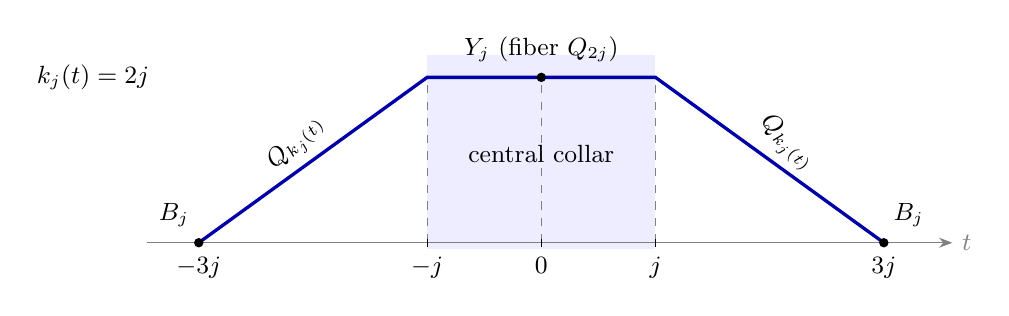
\begin{tikzpicture}[x=1.45cm,y=1.05cm,>=Stealth,font=\small]
 \fill[blue!7] (-1,-0.08) rectangle (1,2.27);
 \draw[->,gray] (-3.45,0)--(3.6,0) node[right] {$t$};
 \draw[very thick,blue!65!black] (-3,0)--(-1,2)--(1,2)--(3,0);
 \draw[dashed,gray] (-1,0)--(-1,2);
 \draw[dashed,gray] (1,0)--(1,2);
 \draw[dashed,gray] (0,0)--(0,2);
 \foreach \x/\lab in {-3/{-3j},-1/{-j},0/{0},1/{j},3/{3j}}{
  \draw (\x,0.05)--(\x,-0.05);
  \node[below] at (\x,-0.06) {$\lab$};
 }
 \fill (-3,0) circle (1.7pt);
 \fill (3,0) circle (1.7pt);
 \fill (0,2) circle (1.7pt);
 \node[above left] at (-3,0.08) {$B_j$};
 \node[above right] at (3,0.08) {$B_j$};
 \node[above] at (0,2.07) {$Y_j$ (fiber $Q_{2j}$)};
 \node at (0,1.08) {central collar};
 \node[rotate=45,above] at (-2,1) {$Q_{k_j(t)}$};
 \node[rotate=-45,above] at (2,1) {$Q_{k_j(t)}$};
 \node[anchor=east] at (-3.35,2) {$k_j(t)=2j$};
\end{tikzpicture}
\caption{The congruence level as a function of height in $X_j$.
Every slice lies over the same discrete torus $B_j$. Outside the central
collar, each vertical step changes the quotient level by one. The drawing
records the level profile, not a geometric embedding of the graph or its
fiber cardinalities.}
\label{fig:profile}
\end{figure}

The gradual reductions in Figure~\ref{fig:profile} have bounded fibers by
Lemma~\ref{geom:quotients}. They therefore preserve a uniform degree bound
even though the middle quotient grows rapidly with $j$.

\begin{lemma}\label{geom:basic}
The graphs $B_j,Y_j,X_j$ are finite and connected, with vertex degrees bounded
independently of $j$. Their projections to $B_j$ are $1$-Lipschitz. Each end
copy of $B_j$ is isometrically embedded in $X_j$.
\end{lemma}

\begin{proof}
Only the claims about $X_j$ remain to be checked. Consecutive slices are
connected by surjective reduction maps, so $X_j$ is connected. A vertex has
at most $|S|$ fiber neighbors, six base neighbors, and at most $2^9$ vertical
neighbors on either side. Thus $|S|+6+2^{10}$ is a common bound. Projection
sends an edge to a base edge or a point, proving the Lipschitz assertion.
Within an end, every base path is available. Projection gives the opposite
distance inequality, so the end metric is exactly the metric of $B_j$.
\end{proof}

\subsection{Coarse disjoint unions}

We now fix metrics on
\[
 B=\bigsqcup_{j\geq1}B_j,\qquad
 Y=\bigsqcup_{j\geq1}Y_j,\qquad
 X=\bigsqcup_{j\geq1}X_j.
\]
In $B_j$ choose the zero vertex, in $Y_j$ the vertex $(0,1)$, and in $X_j$
the vertex $(0,1)$ at height zero. In each union, join the chosen vertices
of components $j$ and $j+1$ by an auxiliary edge of length $100+j^2$, and
use the resulting path distances on the original vertex set. These edges
define the metric; they add no vertices to the space.

A path which leaves and returns to the same component must pass through
its chosen vertex both times. Consequently its use of the auxiliary edges
cannot shorten an intrinsic component distance. At each fixed distance
bound, cross-component pairs occur in only finitely many finite components.
The resulting metrics are uniformly discrete and proper. They have bounded
geometry because the weighted graphs have uniformly bounded degrees and
all edge lengths are at least one: a ball of radius $R$ contains no more
vertices than a ball of graph radius $\lfloor R\rfloor$ in a graph of the
same degree bound.

Projection and end inclusion define maps
\begin{equation}\label{geom:coarse-maps}
 f:Y\longrightarrow B,\qquad i_\pm:B\longrightarrow X.
\end{equation}
On each component they are $1$-Lipschitz. For a fixed input distance bound,
the remaining pairs lie in a finite set, so their image distances also have
a finite bound. Thus the maps are bornologous. Preimages of bounded sets
are finite, so the maps are proper. At scale $3$ none of the Rips complexes
has a cross-component simplex. In particular, the end maps induce proper
simplicial inclusions
\[
 i_{\pm,3}:P_3(B)\longrightarrow P_3(X).
\]
These are the maps used to form the K-homology class. The next section shows
why its two endpoint contributions remain distinct at every fixed scale.

\section{An integral class that persists at every scale}
\label{sec:persistence}

We construct a class $\beta\in\KX_1(B)$ whose images at the two ends of
$X$ have an infinite-order difference. The obstruction to identifying
these images will be integral: at any fixed Rips scale, an appropriate
$K$-cohomology class becomes divisible by larger and larger powers of two
over the middle graphs $Y_j$.

All $K$-groups in this section are complex and integral. For a finite
complex $M$, we write $K^*(M)$ for topological $K$-theory and
$K_*(M)=\KK_*(C(M),\C)$ for analytic $K$-homology. The pairing
\[
 \langle\ ,\ \rangle:K^1(M)\times K_1(M)\longrightarrow\Z
\]
is the Kasparov index pairing. In particular, for a continuous map
$h:M\to N$ between finite complexes,
\begin{equation}
 \langle\eta,h_*\xi\rangle=\langle h^*\eta,\xi\rangle.
 \label{top:pairing-naturality}
\end{equation}
We use the usual Mayer--Vietoris sequence for a finite complex covered
by two subcomplexes; see \cite{HigsonRoe00} for these $K$-homology
constructions.

\subsection{The classes on the two ends}

Let
\[
 T_j=(\R/l_j\Z)^3.
\]
Give $T_j$ its unit cubical subdivision and triangulate the cubes
periodically. The vertices are $B_j$, and the vertices of every cube
have graph distance at most $3$. The resulting triangulated torus is
therefore a subcomplex of $P_3(B_j)$; write
$\kappa_j:T_j\hookrightarrow P_3(B_j)$ for its inclusion.

Let $u_1,u_2,u_3\in H^1(T_j;\Z)$ be the positively oriented coordinate
classes. Choose a line bundle $\mathcal L_j$ pulled back from the first
two circles with
\[
 c_1(\mathcal L_j)=u_1\smile u_2,
\]
and let $e_3\in K^1(T_j)$ be the pullback of the positive generator of
$K^1(S^1)$ under projection to the third circle. Define
\begin{equation}
 \theta_j=([\mathcal L_j]-1)e_3\in K^1(T_j).
 \label{top:theta}
\end{equation}
This class is primitive. Indeed, the exterior-algebra description of
$K^*((S^1)^3)$ identifies $[\mathcal L_j]-1$ with a generator of the
reduced $K^0$ of the first two circles, and $\theta_j$ with the product
of the three circle generators. Here the first assertion also follows
from the first Chern class, which identifies
$\widetilde K^0((S^1)^2)$ with $H^2((S^1)^2;\Z)$.
The K\"unneth and universal coefficient theorems therefore give a class
\begin{equation}
 \tau_j\in K_1(T_j),\qquad
 \langle\theta_j,\tau_j\rangle=1.
 \label{top:tau}
\end{equation}
More explicitly, $K^*(T_j)$ is free abelian, so the universal
coefficient theorem identifies $K_1(T_j)$ with
$\operatorname{Hom}(K^1(T_j),\Z)$, and a primitive element admits an
integer-valued functional taking value $1$ on it; see
\cite[Theorems 23.1.1 and 23.1.3]{Blackadar98}.

The component separation gives
$P_3(B)=\bigsqcup_jP_3(B_j)$. Countable additivity in the first variable
of $\KK$ gives
\begin{equation}
 \KK_1(C_0(P_3(B)),\C)
 \cong\prod_{j\geq1}K_1(P_3(B_j)).
 \label{top:kk-product}
\end{equation}
This is a product, so the entire sequence
$((\kappa_j)_*\tau_j)_j$ determines a class $\beta_3$ in the group on
the left; see \cite[Theorem 19.7.1]{Blackadar98}. Write $\beta$ for its
image in $\KX_1(B)$ and set
\begin{equation}
 \alpha_3=(i_{+,3})_*\beta_3-(i_{-,3})_*\beta_3,
 \qquad
 \alpha=[\alpha_3]\in\KX_1(X).
 \label{top:alpha}
\end{equation}
Thus $\alpha=(i_+)_*\beta-(i_-)_*\beta$. We will prove that every
nonzero integer multiple of $\alpha_3$ remains nonzero at every later
Rips scale.

\subsection{Retractions to the tori}

Fix an integer $r\geq3$. From now on, thresholds on $j$ may depend on
$r$, but not on a simplex or a vertex of the corresponding component.

\begin{lemma}
\label{top:interpolation}
If $l_j>4r$, there is a continuous map
\[
 p_{B,j}:P_r(B_j)\longrightarrow T_j
\]
whose restriction to $T_j\subseteq P_3(B_j)\subseteq P_r(B_j)$ is the
identity. The graph projections define continuous maps
\[
 p_{Y,j}:P_r(Y_j)\longrightarrow T_j,
 \qquad
 p_{X,j}:P_r(X_j)\longrightarrow T_j
\]
by composition with $p_{B,j}$.
\end{lemma}

\begin{proof}
For vertices $u,v$ of a Rips simplex, each coordinate difference has a
unique representative $\delta_i(u,v)\in\Z$ with
$|\delta_i(u,v)|\leq r$. On a triangle $(u,v,w)$, the integer
\[
 \delta_i(u,v)+\delta_i(v,w)-\delta_i(u,w)
\]
is a multiple of $l_j$ and has absolute value at most $3r<l_j$; it
therefore vanishes. Consequently the vertices of each simplex admit
lifts to $\Z^3$ realizing all these differences. The lifts are unique
up to a common element of $l_j\Z^3$. Affine interpolation, followed by
reduction modulo $l_j\Z^3$, gives a map on the simplex independent of
that choice. The maps agree on faces and define $p_{B,j}$.

On each simplex of the triangulated torus, this interpolation is its
original parametrization, so the restriction is the identity. The
projections $Y_j\to B_j$ and $X_j\to B_j$ are $1$-Lipschitz by
Lemma~\ref{geom:basic}; hence they induce simplicial maps of the
corresponding Rips complexes.
\end{proof}

The maps in Lemma~\ref{top:interpolation} allow us to compare the same
torus class at the ends and in the middle. At either end its pairing
with $\tau_j$ is $1$. In the middle, a congruence calculation forces
divisibility.

\subsection{The congruence calculation}

\begin{lemma}
\label{top:chern-divisibility}
For every fixed integer $r\geq3$ and all sufficiently large $j$,
\begin{equation}
 p_{Y,j}^*(u_1\smile u_2)
 \in 2^j H^2(P_r(Y_j);\Z).
 \label{top:chern-divisibility-eq}
\end{equation}
Equivalently, there is a line bundle $\mathcal L'_{j,r}$ on
$P_r(Y_j)$ such that
\begin{equation}
 p_{Y,j}^*\mathcal L_j
 \cong(\mathcal L'_{j,r})^{\otimes 2^j}.
 \label{top:line-root}
\end{equation}
\end{lemma}

\begin{proof}
Take $j$ large enough that $l_j>4r$ and reduction
$\Gamma\to Q_{2j}$ is injective on the word ball of radius $2r$;
the latter condition is available from Lemma~\ref{geom:quotients}.
In this proof write $m=2^j$, suppress $j$ in $U_j,V_j$, and abbreviate
$g_{j,k}$ to $g_k$.

We first describe integral cocycles representing
$p_{Y,j}^*u_1,p_{Y,j}^*u_2$. For an oriented Rips edge $(x,y)$, let
$v_x,v_y\in B_j$ be its projected endpoints and choose their coordinate
representatives in $\{0,\ldots,l_j-1\}$. Define its first two seam
numbers $a_{xy},b_{xy}\in\Z$ by
\[
 \delta_1(v_x,v_y)=(v_y)_1-(v_x)_1+l_j a_{xy},
 \qquad
 \delta_2(v_x,v_y)=(v_y)_2-(v_x)_2+l_j b_{xy}.
\]
The triangle identities in the proof of Lemma~\ref{top:interpolation}
show that $a,b$ are cocycles. The seam numbers record the winding of
the interpolated coordinate maps, so
$[a]=p_{Y,j}^*u_1$ and $[b]=p_{Y,j}^*u_2$.

To prove divisibility by $m$, it suffices to show that $a\smile b$
becomes a coboundary modulo $m$. We will construct a
$\Z/m\Z$-valued $1$-cochain $c$ with $\delta c=-a\smile b$ by
comparing edge transports after lifting from $Q_{2j}$ to $Q_{3j}$.

Order the vertices of $P_r(Y_j)$. For every edge $x<y$, choose a graph
path from $x$ to $y$ of length at most $r$, and write
$x=(v_x,q_x)$ and $y=(v_y,q_y)$. The left Cayley steps along this path
give a word $w_{xy}\in\Gamma$ of length at most $r$. Left
multiplications commute with all horizontal right multiplications.
Moreover, $U,V$ commute modulo $m^2$, and the total seam numbers of the
projected path are $a_{xy},b_{xy}$: its coordinate displacement is
bounded by $r$ and therefore is the unique small lift used above.
It follows that
\begin{equation}
 q_y=\overline w_{xy}\,q_x\,g_{2j}(a_{xy},b_{xy})
 \quad\text{in }Q_{2j}.
 \label{top:edge-transport}
\end{equation}
Here a bar denotes reduction modulo $m^2$.

On an ordered triangle with vertices $x_0<x_1<x_2$, cocycle additivity
and commutation modulo $m^2$ give
\[
 g_{2j}(a_{01},b_{01})g_{2j}(a_{12},b_{12})
 =g_{2j}(a_{02},b_{02}).
\]
Substitution in \eqref{top:edge-transport} and cancellation give
$\overline w_{02}=\overline w_{12}\overline w_{01}$. Both
$w_{02}$ and $w_{12}w_{01}$ lie in the word ball of radius $2r$, so
our injectivity assumption yields the equality in $\Gamma$:
\begin{equation}
 w_{02}=w_{12}w_{01}.
 \label{top:word-triangle}
\end{equation}

We now lift this calculation from modulus $m^2$ to modulus $m^3$.
Every element of
\[
 N=\ker(Q_{3j}\longrightarrow Q_{2j})
\]
has the form $1+m^2D$ modulo $m^3$, with $D$ determined modulo $m$.
Multiplication adds the matrices $D$, since $m^4$ is divisible by
$m^3$. Thus $N$ is abelian and
\[
 d:N\longrightarrow\Z/m\Z,
 \qquad d(1+m^2D)=D_{13}\pmod m
\]
is a homomorphism. Every element of $N$ commutes with every matrix
that is $1$ modulo $m$, in particular with
\[
 \widetilde g(a,b)=V^bU^a\pmod{m^3}.
\]
Direct multiplication of the elementary matrices gives
\begin{equation}
 \begin{split}
 C&=UVU^{-1}V^{-1}=1+m^2E_{13}\pmod{m^3},
       \qquad d(C)=1,\\
 \widetilde g(a,b)\widetilde g(a',b')
   &=\widetilde g(a+a',b+b')C^{ab'}.
 \end{split}
 \label{top:central-extension}
\end{equation}

Choose a lift $\widetilde q_x\in Q_{3j}$ of each $q_x$, and denote the
reduction of $w\in\Gamma$ to $Q_{3j}$ by $\widetilde w$.
Equation~\eqref{top:edge-transport} defines $n_{xy}\in N$ by
\begin{equation}
 \widetilde q_y=
 \widetilde w_{xy}\widetilde q_x
 \widetilde g(a_{xy},b_{xy})n_{xy}.
 \label{top:lifted-edge}
\end{equation}
For an ordered triangle, abbreviate
$\widetilde g(a_{ab},b_{ab})$ to $\widetilde g_{ab}$. Substituting
twice in \eqref{top:lifted-edge} gives
\begin{align*}
 \widetilde q_2
 &=\widetilde w_{12}\widetilde w_{01}\widetilde q_0
       \widetilde g_{01}n_{01}\widetilde g_{12}n_{12}\\
 &=\widetilde w_{02}\widetilde q_0
       \widetilde g_{01}\widetilde g_{12}n_{01}n_{12}\\
 &=\widetilde w_{02}\widetilde q_0\widetilde g_{02}
       C^{a_{01}b_{12}}n_{01}n_{12}.
\end{align*}
The second equality moves $n_{01}$ only past $\widetilde g_{12}$,
which it commutes with; it uses no commutation with
$\widetilde q_0$ or with a Cayley word. Comparing with the direct edge
$02$ therefore gives
\[
 n_{02}=C^{a_{01}b_{12}}n_{01}n_{12}.
\]
Apply $d$ and put $c_{xy}=d(n_{xy})$. With the usual simplicial
coboundary convention, this identity becomes
\[
 (a\smile b)_{012}=a_{01}b_{12}
   =c_{02}-c_{01}-c_{12}=-(\delta c)_{012}
   \quad\text{in }\Z/m\Z.
\]
Hence the reduction of $[a\smile b]$ modulo $m$ is zero. The
cohomology sequence of
\[
 0\longrightarrow\Z\xrightarrow{\,m\,}\Z
   \longrightarrow\Z/m\Z\longrightarrow0
\]
identifies the kernel of reduction on $H^2$ with the image of
multiplication by $m$. This proves
\eqref{top:chern-divisibility-eq}, without a torsion-freeness
assumption on $H^2(P_r(Y_j);\Z)$. Finally, line bundles on a finite
complex are classified by their integral first Chern class, and the
first Chern class of a tensor power is the corresponding integer
multiple. This proves \eqref{top:line-root}.
\end{proof}

\subsection{From line-bundle roots to divisibility in \texorpdfstring{$K^1$}{K1}}

For fixed $r$, bounded geometry supplies an integer $D_r\geq1$ such
that
\[
 \dim P_r(Y_j)\leq D_r\qquad(j\geq1).
\]
Indeed, the vertices of a Rips simplex all belong to the radius-$r$
ball about any one of them, and these balls have uniformly bounded
cardinality. The dimension bound converts the line-bundle roots into
integral divisibility in $K$-theory.

\begin{lemma}
\label{top:k-divisibility}
For every fixed integer $r\geq3$ and all sufficiently large $j$,
\begin{equation}
 p_{Y,j}^*\theta_j\in
 2^{\,j-\lfloor\log_2D_r\rfloor}K^1(P_r(Y_j)).
 \label{top:k-divisibility-eq}
\end{equation}
\end{lemma}

\begin{proof}
Take $j$ satisfying Lemma~\ref{top:chern-divisibility} and $2^j>D_r$,
and put
$z=[\mathcal L'_{j,r}]-1\in K^0(P_r(Y_j))$.
The classifying map of this line bundle can be taken to land in
$\mathbb{CP}^{D_r}$ by cellular approximation. The relation
$([\mathcal H]-1)^{D_r+1}=0$ for the tautological line bundle
$\mathcal H$ on $\mathbb{CP}^{D_r}$ therefore implies
$z^{D_r+1}=0$; see \cite[Corollary 2.7.9]{Atiyah67}.
Consequently \eqref{top:line-root} gives
\begin{equation}
 [p_{Y,j}^*\mathcal L_j]-1
 =(1+z)^{2^j}-1
 =\sum_{h=1}^{D_r}\binom{2^j}{h}z^h.
 \label{top:binomial}
\end{equation}
For $1\leq h\leq D_r$, let $v_2(h)$ be the exponent of $2$ dividing
$h$. The identity
\[
 h\binom{2^j}{h}=2^j\binom{2^j-1}{h-1}
\]
shows that $\binom{2^j}{h}$ is divisible by
$2^{j-v_2(h)}$, hence by
$2^{j-\lfloor\log_2D_r\rfloor}$. Every coefficient in
\eqref{top:binomial} has this common divisor. Multiplying the
resulting divisibility in $K^0$ by $p_{Y,j}^*e_3$ proves the claim.
\end{proof}

We have now obtained the growing divisor over the middle. It remains
to show that an equality between the classes at the two ends would
force their common pairing to have this divisor.

\subsection{Mayer--Vietoris detection and the direct limit}

For $r\geq3$, let
\[
 t_{\pm,j,r}:T_j\longrightarrow P_r(X_j)
\]
denote the inclusion of the triangulated torus at height $\pm3j$.

\begin{lemma}
\label{top:component-detection}
Fix an integer $r\geq3$ and a nonzero integer $n$. For all sufficiently
large $j$,
\begin{equation}
 n(t_{+,j,r})_*\tau_j-n(t_{-,j,r})_*\tau_j
 \neq0\quad\text{in }K_1(P_r(X_j)).
 \label{top:component-nonzero}
\end{equation}
\end{lemma}

\begin{proof}
In addition to the hypotheses needed for
Lemma~\ref{top:k-divisibility}, take $j>2r$. Cover $P_r(X_j)$ by the
induced subcomplexes
\[
 M^+=P_r(X_j)|_{\{t\geq-r\}},\qquad
 M^-=P_r(X_j)|_{\{t\leq r\}},
\]
and put $I=M^+\cap M^-$. These subcomplexes cover: a simplex not
contained in either would contain vertices at heights below $-r$ and
above $r$, contradicting its diameter bound because height is
$1$-Lipschitz. Their intersection is induced on the vertices at heights
in $[-r,r]$.

There is a simplicial map
\[
 h:I\longrightarrow P_r(Y_j)
\]
that forgets height. To check this, join any two vertices in a simplex
of $I$ by a graph path of length at most $r$ in $X_j$. Every vertex of
this path has height in $[-2r,2r]$, which lies in the product collar
since $j>2r$. Forgetting height sends the path to a path in $Y_j$ of
no greater length. Thus the images of the simplex vertices have
diameter at most $r$. The interpolation maps satisfy
\begin{equation}
 p_{X,j}|_I=p_{Y,j}\circ h.
 \label{top:collar-factorization}
\end{equation}

Let $a_\pm:I\hookrightarrow M^\pm$ and
$b_\pm:M^\pm\hookrightarrow P_r(X_j)$ be the inclusions, and write
$t^\pm:T_j\to M^\pm$ for the endpoint inclusions. The relevant part of
the Mayer--Vietoris sequence is
\[
 K_1(I)\xrightarrow{((a_+)_*,-(a_-)_*)}
 K_1(M^+)\oplus K_1(M^-)
 \xrightarrow{(b_+)_*+(b_-)_*}K_1(P_r(X_j)).
\]
If the difference in \eqref{top:component-nonzero} were zero,
exactness would give $\eta\in K_1(I)$ with
\[
 (a_+)_*\eta=n(t^+)_*\tau_j,
 \qquad (a_-)_*\eta=n(t^-)_*\tau_j.
\]
Pair the first equality with $(p_{X,j}|_{M^+})^*\theta_j$. Since
$p_{X,j}\circ t_{+,j,r}=\id_{T_j}$, naturality
\eqref{top:pairing-naturality} and \eqref{top:tau} give
\begin{equation}
 n
 =\langle(p_{X,j}|_I)^*\theta_j,\eta\rangle
 =\langle h^*p_{Y,j}^*\theta_j,\eta\rangle.
 \label{top:divisibility-contradiction}
\end{equation}
By Lemma~\ref{top:k-divisibility}, the last integer is divisible by
$2^{j-\lfloor\log_2D_r\rfloor}$. Taking $j$ large enough that
\[
 j-\lfloor\log_2D_r\rfloor>v_2(|n|)
\]
contradicts \eqref{top:divisibility-contradiction}.
\end{proof}

\begin{proposition}
\label{top:infinite-order}
The class $\alpha\in\KX_1(X)$ defined in \eqref{top:alpha} has infinite
order. In particular, $\alpha\otimes1\neq0$ in
$\KX_1(X)\otimes\mathbb Q$.
\end{proposition}

\begin{proof}
Fix a nonzero integer $n$ and an integer $r\geq3$. Let $\alpha_r$ be
the image of $\alpha_3$ under the map induced by
$P_3(X)\hookrightarrow P_r(X)$. For all sufficiently large $j$, the
component separation ensures that no simplex of $P_r(X)$ meets both
$X_j$ and its complement. Thus $P_r(X_j)$ is a clopen subcomplex, and
extension by zero on functions gives a $*$-homomorphism
\[
 C(P_r(X_j))\longrightarrow C_0(P_r(X)).
\]
Contravariance of $\KK$ in its first variable defines restriction
\[
 \KK_1(C_0(P_r(X)),\C)\longrightarrow K_1(P_r(X_j)).
\]
By \eqref{top:kk-product} and functoriality, the restriction of
$n\alpha_r$ is exactly the difference in
\eqref{top:component-nonzero}. Choosing $j$ also large enough for
Lemma~\ref{top:component-detection} proves $n\alpha_r\neq0$.

We have proved that for every nonzero $n$ and every integer $r\geq3$,
the scale-$r$ image of $n\alpha_3$ is nonzero. If $n\alpha$ vanished
in the filtered direct limit defining $\KX_1(X)$, it would vanish at
some finite later scale; integer scales are cofinal, so this is
impossible. Hence $\alpha$ has infinite order. The kernel of the map
from any abelian group to its tensor product with $\mathbb Q$ is its
torsion subgroup, which proves the final assertion.
\end{proof}

\section{Maximal Roe algebras and the coarse index}
\label{sec:maximal-index}

The infinite-order class is now constructed. It remains to show that its
two end contributions have the same maximal index. The subsequent averaging
and sliding arguments will use operator
formulas on the standard modules.  We therefore establish the norm estimates
that allow those formulas to be used in the maximal completion, and then
verify the required naturality of the index.  These are standard features of
maximal Roe theory; see \cite[Section~2]{OOY09} and
\cite[Section~2]{SS21}.  We give the details needed here because the distinction
between operator norm and maximal norm is essential to the proof.

\subsection{Norm control and multipliers}

Let $Z$ be a uniformly discrete proper metric space of bounded geometry, and
write
\[
 H_0=\ell^2(\N),\qquad H_Z=\ell^2(Z)\otimes H_0,
 \qquad A_Z=C^*_{\max}(Z).
\]
The algebra $\C[Z]$ consists of the bounded finite-propagation operators on
$H_Z$ that are locally compact for the multiplication representation of
$C_0(Z)$.  We denote their concrete operator norm by $\|\cdot\|_{\mathrm{op}}$
and their maximal norm by $\|\cdot\|_{\max}$.  Write $T_{xy}:H_0\to H_0$ for
the matrix entries of an operator $T$.

For a bounded finite-propagation operator, local compactness is equivalent
to compactness of every entry $T_{xy}$.  In one direction, compress by the
characteristic functions of single vertices.  Conversely, every row and
column of a finite-propagation matrix has only finitely many entries.
Multiplication on either side by a finitely supported function therefore
gives a finite matrix of compact operators.  Approximation by finitely
supported functions proves the assertion for every function in $C_0(Z)$.
In particular, no uniform bound on the ranks, or on finite-rank
approximations to the entries, is part of this definition.

\begin{lemma}[Fixed-propagation norm control]
\label{ana:fixed-propagation}
For every $R\geq 0$ there is a constant $c_Z(R)<\infty$ such that
\[
 \|T\|_{\mathrm{op}}\leq\|T\|_{\max}
 \leq c_Z(R)\|T\|_{\mathrm{op}}
 \qquad(T\in\C[Z],\ \prop(T)\leq R).
\]
Consequently, operator-norm convergence of algebraic Roe operators with one
common propagation bound implies convergence in maximal norm.
\end{lemma}

\begin{proof}
Put $N_R=\sup_{z\in Z}|B_Z(z,R)|$.  The support of $T$, viewed as a bipartite
graph with a row copy and a column copy of $Z$, has degree at most $N_R$.
A greedy edge coloring partitions it into at most $2N_R-1$ matchings.
Accordingly, $T=\sum_{a=1}^{2N_R-1}T^{(a)}$, where each $T^{(a)}$ has at most
one nonzero entry in each row and column, and
$\|T^{(a)}\|_{\mathrm{op}}\leq\|T\|_{\mathrm{op}}$.

The diagonal algebra
\[
 \prod_{z\in Z}\mathcal K(H_0)
 =\left\{\operatorname{diag}(k_z): k_z\in\mathcal K(H_0),\
                  \sup_z\|k_z\|<\infty\right\}
\]
is a $C^*$-subalgebra of $\C[Z]$.  Every $*$-representation of $\C[Z]$
restricts to a contractive representation of this algebra.  Since
$(T^{(a)})^*T^{(a)}$ is diagonal, every such representation $\pi$ satisfies
\[
 \|\pi(T^{(a)})\|^2
 \leq\|(T^{(a)})^*T^{(a)}\|_{\mathrm{op}}
 \leq\|T\|_{\mathrm{op}}^2.
\]
The upper bound follows with $c_Z(R)=2N_R-1$.  The concrete representation
on $H_Z$ gives the lower bound.  Apply the estimate to differences to
obtain the convergence assertion.
\end{proof}

This matching argument is the discrete-module form of the maximal-norm
estimate in \cite[Lemma~2.1]{OOY09}; compare
\cite[Lemma~1.10]{SW13}.  We shall also use the following stronger statement
when the vertex support, rather than merely the propagation, is fixed.

\begin{lemma}[The compact ideal]
\label{ana:compacts}
An operator in $\C[Z]$ supported on $F\times F$, for a finite set $F\subset Z$,
has the same maximal and concrete norms.  The closure in $A_Z$ of all such
operators is an ideal $\mathcal K_Z$, canonically isomorphic to
$\mathcal K(H_Z)$.  In particular, $K_1(\mathcal K_Z)=0$.
\end{lemma}

\begin{proof}
The operators supported on $F\times F$ form the $C^*$-algebra
$\mathcal K(\ell^2(F)\otimes H_0)$.  Restriction of any representation is
contractive, and the concrete representation gives the reverse inequality.
These finite-vertex algebras have dense union in $\mathcal K(H_Z)$.
Multiplying one of their elements on either side by a finite-propagation
operator with compact entries gives another compact operator of finite
vertex support: only a finite metric neighborhood of $F$ can occur.
Density proves the ideal assertion.
\end{proof}

We will need finite-propagation operators whose entries are bounded but
need not be compact, such as the unitaries implementing the group action.
Here and below $M(A_Z)$ denotes the multiplier algebra of $A_Z$.

\begin{lemma}[Finite-propagation multipliers]
\label{ana:multipliers}
Every bounded finite-propagation operator $D$ on $H_Z$ acts by left and
right multiplication on $\C[Z]$, and these actions extend to a multiplier
of $A_Z$.  This assignment is a faithful $*$-homomorphism and satisfies
\[
 \|D\|_{\mathrm{op}}\leq \|D\|_{M(A_Z)}
 \leq c_Z(R)\|D\|_{\mathrm{op}}
 \qquad\text{if }\prop(D)\leq R.
\]
For an operator supported on a single matching, the multiplier norm equals
the concrete norm.
\end{lemma}

\begin{proof}
Products of $D$ with elements of $\C[Z]$ have finite propagation and compact
entries.  Decompose $D$ into matchings as in
Lemma~\ref{ana:fixed-propagation}.  It suffices to show that a matching
operator whose entries have norm at most one acts contractively.
For such an operator, $D^*D$ is a diagonal positive contraction.  The
operator $W=(1-D^*D)^{1/2}$ is bounded and diagonal.  For $T\in\C[Z]$,
all terms in
\[
 T^*T-(DT)^*(DT)=(WT)^*(WT)
\]
belong to $\C[Z]$.  Applying each $*$-representation gives
$\|DT\|_{\max}\leq\|T\|_{\max}$.  Applying this to $D^*$ and taking
adjoints gives the corresponding right-multiplication bound.  The
algebraic compatibility identities between these left and right actions
pass to the completion, so they define a multiplier.  Summing the
matching estimates gives the asserted upper bound.

The assignment preserves products and adjoints on the dense algebra
$\C[Z]$.  The concrete representation of $A_Z$ on $H_Z$ is nondegenerate,
since it contains $\mathcal K(H_Z)$, and hence extends to the multiplier
algebra.  It sends the multiplier just constructed to the original
operator $D$, proving the lower bound and faithfulness.
\end{proof}

In particular, an operator identity involving bounded finite-propagation
operators remains an identity between their multipliers.  This statement
does not assert that the concrete representation of the entire maximal
Roe algebra is faithful.  The finite-propagation control in the preceding
lemmas is what will justify the specific limits below.

\subsection{Maps induced by coarse maps}

A map $h:Z\to W$ between uniformly discrete proper bounded-geometry spaces
is coarse if inverse images of bounded sets are bounded and, for every
$R$, there is $S$ such that $d_Z(x,y)\leq R$ implies
$d_W(h(x),h(y))\leq S$.  Choose an isometry
$V_h:H_Z\to H_W$ that sends the summand over $z$ into the summand over
$h(z)$, using orthogonal ranges when several vertices have the same image.
Such a choice is possible because the vertex fibers are finite and $H_0$
is infinite dimensional.  We call $V_h$ an exact covering isometry for $h$.

\begin{proposition}[Coarse functoriality]
\label{ana:functoriality}
Conjugation by an exact covering isometry defines a $*$-homomorphism
\[
 h_A=\Ad(V_h):A_Z\longrightarrow A_W.
\]
Its induced map on $K$-theory is independent of the covering isometry.
These induced maps respect composition, and an exact covering isometry
over $\id_Z$ induces the identity on $K_*(A_Z)$.
\end{proposition}

\begin{proof}
For $T\in\C[Z]$, coarse control bounds the propagation of $V_hTV_h^*$.
Each of its vertex entries is a finite sum of compact operators, because
$h^{-1}(w)$ is finite for each $w$.  Thus conjugation is a $*$-homomorphism
$\C[Z]\to\C[W]$, and the universal property extends it contractively to
the maximal completions.

For two choices $V_0,V_1$, put
\[
 V_\lambda=
 \begin{pmatrix}\cos\lambda\,V_0\\ \sin\lambda\,V_1\end{pmatrix}
 :H_Z\longrightarrow H_W\oplus H_W,
 \qquad 0\leq\lambda\leq\pi/2.
\]
Each $V_\lambda$ is an isometry.  Conjugation defines a homomorphism to
$M_2(A_W)$: its four matrix entries have compact vertex entries and one
common propagation bound for every fixed $T\in\C[Z]$.  Moreover,
\[
 \|V_\lambda T V_\lambda^*-V_\nu T V_\nu^*\|_{\mathrm{op}}
 \leq 2\|T\|_{\mathrm{op}}|\lambda-\nu|.
\]
Lemma~\ref{ana:fixed-propagation}, applied to the four entries, promotes
this estimate to maximal-norm continuity on $\C[Z]$; contractivity and
density give continuity on $A_Z$.  The two endpoint homomorphisms are
$\Ad(V_0)$ and $\Ad(V_1)$ in the two standard matrix corners, which induce
the same stabilized $K$-theory map.  Composing covering isometries proves
functoriality, and comparison with the identity isometry proves the last
assertion.
\end{proof}

This is the exact-covering version of \cite[Lemma~2.15]{OOY09}.  For the
maps in our construction we henceforth choose such homomorphisms and write
\[
 f_A:A_Y\longrightarrow A_B,\qquad
 i_{\pm,A}:A_B\longrightarrow A_X.
\]
By Proposition~\ref{ana:functoriality}, all statements about their
$K$-theory maps are independent of these choices.

\subsection{The canonical odd index and naturality}

The remaining index-theoretic input is compatibility with the two end
inclusions.

\begin{proposition}[Naturality for the end classes]
\label{ana:naturality}
For the classes $\beta\in\KX_1(B)$ and
$\alpha=(i_+)_*\beta-(i_-)_*\beta\in\KX_1(X)$ constructed above,
\begin{equation}
 \label{eq:ana-naturality}
 \mu_X^{\max}(\alpha)
 =(i_{+,A})_*\mu_B^{\max}(\beta)
  -(i_{-,A})_*\mu_B^{\max}(\beta).
\end{equation}
\end{proposition}

To verify this identity in the maximal completion, we first identify the
Roe algebra of a Rips complex with the vertex algebra and then recall the
exponential formula for its canonical odd index.

For $r>0$, regard a point of $P_r(Z)$ as a finitely supported probability
measure on $Z$ whose support has diameter at most $r$.  Equip the complex
with the $1$-Wasserstein metric induced by $d_Z$.  Every point is within
$r$ of every vertex of its support.  Moreover, a bounded set in this
metric uses only vertices from one bounded subset of $Z$: if $v$ is a
support vertex of $p$, then
\[
 d_Z(v,z_0)\leq r+\int_Z d_Z(z,z_0)\,dp(z)
             =r+d_{W_1}(p,\delta_{z_0}).
\]
That subset is finite.  Consequently this metric is proper and induces
the usual topology on the locally finite complex.  The vertex inclusion
and any selection of a support vertex are coarse inverses.

Choose a countable dense subset $E\subset P_r(Z)$ containing the vertices,
and use the ample module $\ell^2(E)\otimes H_0$ with pointwise
multiplication by $C_0(P_r(Z))$.  Assign each point of $E$ to one vertex of
its support, assigning a vertex to itself.  This partitions the module
into infinite-dimensional separable blocks $H_v$, one for each $v\in Z$;
choose identifications $H_v\cong H_0$.

Under this regrouping, the algebraic Roe algebra of $P_r(Z)$ is exactly
$\C[Z]$.  Propagation bounds in the two descriptions differ by at most
$2r$.  For local compactness, the points in $H_v$ lie in the compact
closed star of $v$, so a compactly supported continuous cutoff equal to
one on that star shows that a locally compact operator has compact
vertex-block entries.  Conversely, a compact subset of $P_r(Z)$ meets
only finitely many blocks.  Compact vertex-block entries and finite
propagation therefore give local compactness after multiplication by a
compactly supported function, and then by any function in $C_0(P_r(Z))$.
The algebraic identification extends to the maximal completions by
universality.  It is the coarse identification induced by the chosen
support-vertex map.  Pseudolocality below is always taken relative to
$C_0(P_r(Z))$; the regrouping is used only for the Roe algebra and for
Lemma~\ref{ana:multipliers}.

We recall the cycle description of the odd index.  On an ample module
for $P_r(Z)$, an odd $K$-homology class is represented, after stabilization
and addition of degenerate cycles, by a bounded self-adjoint operator
$F$ such that
\[
 [F,a]\text{ is compact},\qquad a(F^2-1)\text{ is compact}
 \quad(a\in C_0(P_r(Z))).
\]
The first condition is pseudolocality.  The use of a fixed ample module
is the usual Paschke realization of locally finite $K$-homology; see
\cite{HigsonRoe00}.

Such a representative may be taken to have finite propagation.  Indeed,
let $\varphi_v$ be the square roots of the barycentric coordinate
functions.  Their supports are compact, have diameter at most $2r$,
and form a locally finite family with $\sum_v\varphi_v^2=1$.  Set
\[
 F'=\sum_v\varphi_vF\varphi_v.
\]
The sum converges strongly and has norm at most $\|F\|$: it is the
compression of the direct sum of copies of $F$ by the isometry
$\xi\mapsto(\varphi_v\xi)_v$.  It has propagation at most $2r$.
Furthermore,
\[
 F'-F=\sum_v\varphi_v[F,\varphi_v]
\]
is locally compact, since multiplication on the left by a compactly
supported function leaves only finitely many compact summands; use
self-adjointness for the right-hand assertion.  Thus the straight-line
path from $F$ to $F'$ consists of cycles and does not change the
$K$-homology class.  Replace $F$ by $F'$.

After regrouping into vertex blocks, Lemma~\ref{ana:multipliers} makes
$F$ a self-adjoint multiplier of $A_Z$, and finite propagation gives
$F^2-1\in\C[Z]$.  Hence
\[
 p=\frac{1+F}{2}\in M(A_Z),\qquad
 p^2-p\in\C[Z],\qquad
 u_F=\exp(2\pi i p)\in 1+A_Z.
\]
The odd maximal index is
\begin{equation}
 \label{eq:ana-odd-index}
 \operatorname{Ind}_{Z,\max}(F)=[u_F]\in K_1(A_Z).
\end{equation}
To relate this formula to the canonical index, let
$D^*_{\max}(P_r(Z))$ be the universal completion of the algebra of
finite-propagation pseudolocal operators on the Rips module.  It contains
$A_Z$ as an ideal, and Paschke duality identifies
\[
 \KK_1(C_0(P_r(Z)),\C)
 \cong K_0\bigl(D^*_{\max}(P_r(Z))/A_Z\bigr),
 \qquad [F]\longmapsto[p\bmod A_Z].
\]
These assertions, including existence of the universal completion, are
proved in \cite[Proposition~2.22, Propositions~2.27--2.28, and
Corollary~2.29]{SS21}.  The index is the boundary map of this extension.
The multiplier action of Lemma~\ref{ana:multipliers} agrees with the
inclusion on $A_Z$, so its exponential boundary formula is exactly
\eqref{eq:ana-odd-index}.  Thus this formula computes the canonical index,
with its usual boundary-map sign convention.  It agrees with the cycle
construction in \cite[Corollary~2.18]{OOY09}.  Passing to the Rips direct
limit gives $\mu_Z^{\max}$.



\begin{proof}[Proof of Proposition~\ref{ana:naturality}]
Both classes are represented at Rips scale $3$, where the end maps are
proper continuous coarse simplicial inclusions
$i_{\pm,3}:P_3(B)\to P_3(X)$.  Choose the dense-set modules compatibly:
the target dense set contains the images of the source dense set, and
the support-vertex choices agree on these images.  The resulting module
isometry $V$ is an exact covering isometry for the end map after
regrouping.

If $F$ represents a source odd class and has finite propagation, its
push-forward is represented on the target module by
\[
 \widetilde F=VFV^*-(1-VV^*).
\]
The complement is a degenerate cycle.  Properness ensures that pullbacks
of $C_0$ functions lie in $C_0$, so $\widetilde F$ is pseudolocal and
$\widetilde F^2-1$ is locally compact.  Coarse control preserves finite
propagation.  Writing $p=(1+F)/2$, we have
$\widetilde p=(1+\widetilde F)/2=VpV^*$.

For completeness, compatibility of the exponential with conjugation
holds in the maximal completion itself.  The function
\[
 h(z)=\frac{\exp(2\pi i z)-1}{z^2-z}
\]
extends to an entire function.  Approximate $h$ uniformly by polynomials
on disks containing the spectra of the two multipliers.  Since
\[
 \exp(2\pi i p)-1=(p^2-p)h(p),
\]
and $p^2-p\in\C[B]$, all polynomial identities are identities on the
algebraic Roe algebras, and their limits hold in maximal norm.  They give
\[
 \exp(2\pi i\widetilde p)-1
   =i_{\pm,A}\bigl(\exp(2\pi i p)-1\bigr).
\]
Thus the two indices commute with the end inclusion.  Apply this to
$\beta_3$, subtract the two identities, and use the definition of the
Rips direct-limit assembly map.  Independence of the covering choices
follows from Proposition~\ref{ana:functoriality}.
\end{proof}

\section{A transfer in the maximal Roe algebra}\label{sec:transfer}

The projection $f:Y\to B$ forgets a finite Cayley graph over each base
vertex.  We will lift operators on $B$ to operators on $Y$ by transporting
their matrix entries between these fibers and then projecting onto the
constant vectors.  The resulting map supplies the analytic class that we
will move from one end of $X$ to the other.

\begin{proposition}\label{ana:transfer}
For the projection $f:Y\to B$ there is a $*$-homomorphism
\[
 \Phi:A_B\longrightarrow A_Y
\]
such that $(f_A\Phi)_*=\id$ on $K_*(A_B)$.  In particular,
\[
 (f_A)_*:K_1(A_Y)\longrightarrow K_1(A_B)
\]
is surjective.
\end{proposition}

Throughout this section, $u,v,w$ denote vertices of $B$.  Write
$F_u=f^{-1}(u)$ and let
\[
 \xi_u=|F_u|^{-1/2}\sum_{y\in F_u}\delta_y
 \quad\text{in }\ell^2(F_u).
\]
These vectors define an isometry
\begin{equation}\label{eq:constant-isometry}
 V:H_B\longrightarrow H_Y,
 \qquad V(\delta_u\otimes h)=\xi_u\otimes h.
\end{equation}
The diameters of the fibers are not uniformly bounded, so $V$ itself need
not be a covering isometry for a coarse map.  We will obtain an element of
the maximal Roe algebra from this averaging operation by using
property~\textup{(T)}.

\subsection{The projection onto fiber constants}

For $\gamma\in\Gamma$, let $U_\gamma$ act by left multiplication by
$\gamma$ on every fiber, with the identity on $H_0$.  This is a unitary
operator of propagation at most the word length of $\gamma$.
Lemma~\ref{ana:multipliers} therefore gives a unitary representation
\[
 \Gamma\longrightarrow M(A_Y),\qquad\gamma\longmapsto U_\gamma,
\]
and hence a unital $*$-homomorphism from $C^*_{\max}(\Gamma)$ into
$M(A_Y)$.

We recall explicitly the consequence of property~\textup{(T)} that will
be used; see \cite{BHV08}.  In $C^*_{\max}(\Gamma)$ put
\[
 \Delta=1-\frac1{|S|}\sum_{s\in S}s.
\]
For every unitary representation $\pi$ and every vector $\eta$,
\[
 \langle\pi(\Delta)\eta,\eta\rangle
   =\frac1{2|S|}\sum_{s\in S}
      \|\pi(s)\eta-\eta\|^2.
\]
In particular, $0\le\Delta\le2$, and the kernel of $\pi(\Delta)$ is
the invariant subspace.  Property~\textup{(T)}, applied to the fixed finite
generating set $S$, gives $\kappa>0$ such that every unit vector
orthogonal to that subspace is moved by at least $\kappa$ by some
$s\in S$.  Consequently, with $\varepsilon=\kappa^2/(2|S|)$,
\[
 \sigma_{C^*_{\max}(\Gamma)}(\Delta)
     \subseteq\{0\}\cup[\varepsilon,2].
\]
The continuous functional calculus thus gives a projection onto the
invariant vectors in every representation, and
\[
 \left(1-\frac{\Delta}{2}\right)^n
\]
converges to this projection in the maximal group norm.  Denote its image
in $M(A_Y)$ by $P$, and denote the images of the displayed approximants
by $P_n$.  We have
\begin{equation}\label{eq:kazhdan-convergence}
 \|P_n-P\|_{M(A_Y)}\longrightarrow0.
\end{equation}
Each $P_n$ is a finite-propagation multiplier preserving every fiber.

In the concrete representation on $H_Y$, the invariant vectors in
$\ell^2(F_u)$ are precisely the constant vectors: the map
$\Gamma\to Q_{2j}$ is onto and its left action on $F_u$ is transitive.
Thus the concrete image of $P$ is $VV^*$. The transfer itself will use
$P$ in the maximal multiplier algebra $M(A_Y)$.

\subsection{Transporting matrix entries}

For each pair $u,v$ in the same component $B_j$, choose a shortest edge
path from $v$ to $u$, choosing the reverse path for the reversed pair.
Horizontal transport along this path is a permutation
\[
 O_{uv}:\ell^2(F_v)\longrightarrow\ell^2(F_u).
\]
Take $O_{uu}=1$.  When $u,v$ lie in different components, instead put
\[
 O_{uv}=|\xi_u\rangle\langle\xi_v|.
\]
In both cases,
\begin{equation}\label{eq:transport-constants}
 O_{vu}=O_{uv}^*,\qquad
 O_{uv}\xi_v=\xi_u,\qquad O_{uv}^*\xi_u=\xi_v.
\end{equation}
Moreover, $O_{uv}$ intertwines the left $\Gamma$-actions.  For
horizontal transport this follows because the matchings use right
multiplication; for the rank-one operators it follows because both
vectors are invariant.

Given $T\in\C[B]$, use the decomposition
$H_Y=\bigoplus_{u\in B}\ell^2(F_u)\otimes H_0$ to define
\begin{equation}\label{eq:transport-lift}
 L(T)_{uv}=O_{uv}\otimes T_{uv}.
\end{equation}
This is a linear, adjoint-preserving lift, but it need not be
multiplicative.  The next lemma isolates both its control and the precise
failure of multiplicativity.

\begin{lemma}\label{ana:transport-defect}
For $T\in\C[B]$, the operator $L(T)$ belongs to $\C[Y]$ and commutes
with $P$.  For $T,T'\in\C[B]$, the defect
\begin{equation}\label{eq:transport-defect}
 D=L(T)L(T')-L(TT')
\end{equation}
has finite vertex support and satisfies $PD=0$ in $A_Y$.
\end{lemma}

\begin{proof}
Let $R$ be a propagation bound for $T$.  The matrix support of $T$ can
be partitioned into finitely many matchings of the base vertices, with a
number depending only on $R$ and the bounded geometry of $B$.  On one
such matching, the blocks in \eqref{eq:transport-lift} have disjoint
domain and range blocks, and their norms are at most $\|T\|_{\mathrm{op}}$.
Summing over the matchings proves that $L(T)$ is bounded.

Within a component, any nonzero vertex entry of $O_{uv}$ joins vertices
connected by the chosen horizontal path.  Its length is
$d_B(u,v)\le R$.  Among different components, only finitely many vertex
pairs $(u,v)$ can occur at this propagation bound; their fibers are
finite.  The remaining entries therefore also have a finite propagation
bound.  Each vertex entry of $L(T)$ is a scalar multiple of a compact
operator $T_{uv}$.  It follows that $L(T)\in\C[Y]$.
The intertwining property of $O_{uv}$ shows that $L(T)$ commutes with
every $U_\gamma$, hence with every $P_n$ and with $P$.

We next locate the defect.  Let $R'$ be a propagation bound for $T'$.
Outside finitely many components, all entries involved in
\eqref{eq:transport-defect} stay in a single component $B_j$.
For a summand with intermediate vertex $v$, the concatenated path from
$w$ to $v$ to $u$ has length at most $R+R'$, as does the chosen path
from $w$ to $u$.  If $l_j>2(R+R')$, these two paths have the same total
seam crossing numbers.  Indeed, their lifted coordinate displacements
differ by a multiple of $l_j$ and have difference of absolute value at
most $2(R+R')$ in each coordinate.  That multiple must be zero.
Since $U_j$ and $V_j$ commute in $Q_{2j}$, horizontal transport depends
only on these seam totals.  It follows that
\[
 O_{uv}O_{vw}=O_{uw}
\]
for every summand under consideration.  The defect therefore vanishes
on all sufficiently large components.  The omitted components and any
cross-component entries lie in a finite union of finite graphs, so $D$
has finite vertex support.

Equations~\eqref{eq:transport-constants} give, on the concrete Hilbert
spaces,
\[
 L(T)V=VT,\qquad V^*L(T)=TV^*.
\]
The concrete image of $PD$ is consequently zero.  To obtain the equality
in the maximal completion, choose a finite union $E$ of components of
$Y$ containing the vertex support of $D$.  Every $P_n$ preserves each
fiber, so $P_nD$ has vertex support in the same finite set $E$.
Lemma~\ref{ana:compacts} identifies its maximal norm with its concrete
operator norm.  On $H_Y$, we have $P_nD\to0$ in operator norm; hence
$P_nD\to0$ in maximal norm.  On the other hand,
\eqref{eq:kazhdan-convergence} gives $P_nD\to PD$ in $A_Y$.
Thus $PD=0$ in $A_Y$.
\end{proof}

\subsection{The splitting}

We can now define the transfer and compute its composition with $f_A$.
The first task used finite vertex support.  The second will use a
different control: averaging can increase propagation inside a fiber,
but it does not increase propagation after the fiber is projected to its
base vertex.

\begin{proof}[Proof of Proposition~\ref{ana:transfer}]
For $T\in\C[B]$, put
\[
 \Phi(T)=PL(T)\in A_Y.
\]
Since $P$ is a projection commuting with the lifts,
Lemma~\ref{ana:transport-defect} gives
\[
 \Phi(T)\Phi(T')=P L(T)L(T')=P L(TT')=\Phi(TT').
\]
The lift preserves adjoints, so $\Phi$ is a $*$-homomorphism on
$\C[B]$.  The universal property of the maximal norm extends it to a
$*$-homomorphism $A_B\to A_Y$.

Let $J:H_Y\to H_B$ be the covering isometry defining $f_A$; it sends
the summand at $y\in F_u$ isometrically into the summand at $u$, with
orthogonal ranges for distinct $y$ in the same fiber.  For
$T\in\C[B]$, continuity gives
\begin{equation}\label{eq:split-approximants}
 f_A\Phi(T)=\lim_{n\to\infty} J P_nL(T)J^*
 \qquad\text{in }A_B.
\end{equation}
All operators in this limit have propagation at most $\prop(T)$ on
$B$, because $P_n$ preserves the fibers.  In concrete operator norm
they converge to
\[
 JVV^*L(T)J^*=JVT V^*J^*.
\]
The isometry $JV:H_B\to H_B$ lies over the identity of $B$, so
$JVT V^*J^*$ belongs to $\C[B]$ and has the same propagation bound.
The difference from each approximant in
\eqref{eq:split-approximants} has this fixed propagation bound as well.
Lemma~\ref{ana:fixed-propagation} promotes the concrete convergence to
maximal-norm convergence.  Hence
\begin{equation}\label{eq:split-identity}
 f_A\Phi(T)=\Ad(JV)(T).
\end{equation}
By density this identity holds on $A_B$.
Finally, Proposition~\ref{ana:functoriality} says that a covering isometry
over the identity induces the identity on $K$-theory.  Applying it to
$JV$ proves $(f_A\Phi)_*=\id$.
\end{proof}

\section{Moving the analytic class to the two ends}\label{sec:sliding}

The two endpoint maps $i_-f,i_+f:Y\to X$ are connected componentwise
by the height slices of $X_j$.  The distance between the endpoints grows
with $j$, so a single bounded-distance homotopy does not compare their
Roe-algebra maps.  Instead, we place a copy of an operator at every
height and compare this stack with its shift by one height.  The common
interior copies will cancel on $K$-theory.

\begin{proposition}\label{ana:endpoints}
The endpoint maps induce the same homomorphism
\[
 (i_{+,A}f_A)_*=(i_{-,A}f_A)_*:
 K_1(A_Y)\longrightarrow K_1(A_X).
\]
\end{proposition}

For $-3j\le t\le3j$, let
\[
 s_{j,t}:Y_j\longrightarrow X_j,
 \qquad (u,q)\longmapsto (u,\overline q,t),
\]
where $\overline q$ is reduction from $Q_{2j}$ to $Q_{k_j(t)}$.
The map is $1$-Lipschitz: it carries both Cayley edges and horizontal
matchings to edges or to vertices.  Consecutive slices satisfy
\begin{equation}\label{eq:successive-slices}
 d_X(s_{j,t}(y),s_{j,t+1}(y))=1.
\end{equation}
Choose exact covering isometries
\[
 D_{j,t}:H_{Y_j}\longrightarrow H_{X_j}
\]
over these vertex maps.  They exist because every vertex summand is a
copy of the infinite-dimensional Hilbert space $H_0$.  At the endpoints
choose them to be the restrictions of the covering isometries defining
$i_{-,A}f_A$ and $i_{+,A}f_A$, respectively.  For fixed $j$, the ranges
of the $D_{j,t}$ for distinct $t$ are orthogonal, since they lie at
distinct heights.

\subsection{Stacks modulo the compact operators}

Let
\[
 q:A_X\longrightarrow A_X/\K_X
\]
be the quotient map.  If $T\in\C[Y]$, write
$T_j=\chi_{Y_j}T\chi_{Y_j}$.  The difference
$T-\bigoplus_jT_j$ has finite vertex support: at a fixed propagation
bound there are only finitely many cross-component entries.  In
particular it is compact.  Define
\begin{align}
 S_0(T)&=\bigoplus_j\sum_{t=-3j}^{3j-1}
                D_{j,t}T_jD_{j,t}^*,\label{eq:stack-zero}\\
 S_1(T)&=\bigoplus_j\sum_{t=-3j}^{3j-1}
                D_{j,t+1}T_jD_{j,t+1}^*.
                \label{eq:stack-one}
\end{align}
The number of copies is unbounded, but their ranges are orthogonal.
Thus $\|S_a(T)\|_{\mathrm{op}}\le\|T\|_{\mathrm{op}}$, for $a=0,1$.
If $\prop(T)\le R$, the $1$-Lipschitz property gives
$\prop(S_a(T))\le R$.
Every vertex entry is compact: it is a finite sum of isometric images
of compact entries of $T_j$, since each $Y_j$ is finite.  Hence
$S_a(T)\in\C[X]$.  No bound on the ranks of these compact entries is
required in the algebra used here.

The maps $S_a$ need not be multiplicative before taking the quotient.
For $T,T'\in\C[Y]$, however,
\begin{equation}\label{eq:compression-defect}
 (TT')_j-T_jT'_j
   =\chi_{Y_j}T(1-\chi_{Y_j})T'\chi_{Y_j}
\end{equation}
is zero except for finitely many $j$.  Each nonzero term is compact on
$H_{Y_j}$, since it is a matrix of compact operators over a finite
vertex set.  Copying it into the finitely many heights of the
corresponding $X_j$ remains compact.  Orthogonality of the height
ranges and \eqref{eq:compression-defect} therefore show that
\[
 \overline S_a=qS_a:\C[Y]\longrightarrow A_X/\K_X
\]
is a $*$-homomorphism.  By maximal universality, it extends to a
$*$-homomorphism with domain $A_Y$.

\subsection{A continuous rotation between the stacks}

We next prove that $\overline S_0$ and $\overline S_1$ induce the same
map on $K$-theory.  The rotation takes place in a doubled target module;
this ensures that the ranges stay orthogonal at every intermediate
angle.

For $0\le\lambda\le\pi/2$, define
\[
 W_{\lambda,j,t}=
 \begin{pmatrix}
  \cos\lambda\,D_{j,t}\\
  \sin\lambda\,D_{j,t+1}
 \end{pmatrix}
 :H_{Y_j}\longrightarrow H_{X_j}\oplus H_{X_j},
 \qquad -3j\le t<3j.
\]
Each $W_{\lambda,j,t}$ is an isometry.  For distinct pairs $(j,t)$,
their ranges are orthogonal: they lie in different components or, within
one component, at different heights in each target copy.  In the first
copy the heights are $t$, and in the second they are $t+1$.
Thus they assemble to an
isometry
\[
 W_\lambda:\bigoplus_{j}\bigoplus_{t=-3j}^{3j-1}H_{Y_j}
          \longrightarrow H_X\oplus H_X.
\]
On $\C[Y]$ define
\begin{equation}\label{eq:stack-rotation}
 F_\lambda(T)=W_\lambda
       \left(\bigoplus_j\bigoplus_{t=-3j}^{3j-1}T_j\right)
       W_\lambda^*.
\end{equation}
Its diagonal matrix blocks are scalar multiples of the stacks in
\eqref{eq:stack-zero}--\eqref{eq:stack-one}.  The off-diagonal blocks
are sums of $D_{j,t}T_jD_{j,t+1}^*$ and their counterparts.  If
$\prop(T)\le R$, then \eqref{eq:successive-slices} gives propagation
at most $R+1$ for these blocks.  Their vertex entries are again finite
sums of compact operators.  We conclude that
\[
 F_\lambda(T)\in M_2(\C[X]),\qquad
 \prop(F_\lambda(T))\le R+1.
\]
The same calculation as \eqref{eq:compression-defect}, using
$W_\lambda^*W_\lambda=1$, shows that the images of $F_\lambda$ in
$M_2(A_X/\K_X)$ are $*$-homomorphisms on $\C[Y]$.  Each extends to
$A_Y$ by maximal universality.

For completeness, continuity is uniform in the number of height
slices.  The orthogonality just established gives
\[
 \|W_\lambda-W_\mu\|
  =\bigl((\cos\lambda-\cos\mu)^2
            +(\sin\lambda-\sin\mu)^2\bigr)^{1/2}
  \le |\lambda-\mu|.
\]
Consequently, in concrete operator norm,
\begin{equation}\label{eq:rotation-continuity}
 \|F_\lambda(T)-F_\mu(T)\|_{\mathrm{op}}
       \le2\|T\|_{\mathrm{op}}\,|\lambda-\mu|.
\end{equation}
The difference has propagation at most $R+1$, independently of the
angles.  Applying Lemma~\ref{ana:fixed-propagation} to its four matrix
blocks promotes \eqref{eq:rotation-continuity} to an estimate
\[
 \|F_\lambda(T)-F_\mu(T)\|_{M_2(A_X)}
       \le C_R\|T\|_{\mathrm{op}}\,|\lambda-\mu|
\]
for a constant independent of $j,\lambda,\mu$.
This proves point-norm continuity on the dense algebra $\C[Y]$.
The extended homomorphisms are contractive for the maximal norm, so
density proves point-norm continuity on all of $A_Y$.

At $\lambda=0$ the homomorphism is $\overline S_0$ in the first
matrix corner, and at $\lambda=\pi/2$ it is $\overline S_1$ in the
second.  The corner identifications on $K$-theory agree, so
\begin{equation}\label{eq:equal-stacks}
 (\overline S_0)_*=(\overline S_1)_*.
\end{equation}

\subsection{Canceling the interior copies}

\begin{proof}[Proof of Proposition~\ref{ana:endpoints}]
Define the interior stack by
\[
 I(T)=\bigoplus_j\sum_{t=-3j+1}^{3j-1}D_{j,t}T_jD_{j,t}^*.
\]
Its image $\overline I=qI$ is a $*$-homomorphism on $A_Y$ by the
same compact-defect argument.  Let
\[
 E_-=i_{-,A}f_A,\qquad E_+=i_{+,A}f_A.
\]
The endpoints in the two stacks agree modulo $\K_X$ with $E_-$ and
$E_+$, respectively.  Indeed, our endpoint covering isometries agree
with those defining $E_\pm$, and discarding the cross-component part
of $T$ changes its image by a compact operator.  Hence
\[
 \overline S_0=\overline I+qE_-,\qquad
 \overline S_1=\overline I+qE_+.
\]
In each sum, the two homomorphisms have orthogonal ranges: one is
supported on the strictly interior heights and the other on an
endpoint.

Orthogonal sums induce sums on $K_1$.  Explicitly, if $\varphi$ and
$\psi$ are orthogonal homomorphisms and $u$ is a matrix unitary with
$u-1$ in the domain algebra, then
\[
 1+(\varphi+\psi)(u-1)
   =\bigl(1+\varphi(u-1)\bigr)
      \bigl(1+\psi(u-1)\bigr),
\]
and multiplication of unitaries gives addition of their $K_1$-classes.
Using this additivity in \eqref{eq:equal-stacks} and canceling
$\overline I_*$ gives
\[
 q_*(E_-)_*=q_*(E_+)_*.
\]
By Lemma~\ref{ana:compacts}, $\K_X$ is the algebra of compact
operators on $H_X$, so $K_1(\K_X)=0$.  The six-term exact sequence
for
\[
 0\longrightarrow\K_X\longrightarrow A_X
       \xrightarrow{q}A_X/\K_X\longrightarrow0
\]
therefore makes $q_*:K_1(A_X)\to K_1(A_X/\K_X)$ injective.
It follows that $(E_-)_*=(E_+)_*$, as asserted.
\end{proof}

\begin{proof}[Proof of Theorem~\ref{thm:main}]
The graphs $X_j$ constructed above are finite and connected with a
uniform degree bound, and their coarse disjoint union $X$ is uniformly
discrete and has bounded geometry.  Proposition~\ref{top:infinite-order}
gives an infinite-order class
\[
 \alpha=(i_+)_*\beta-(i_-)_*\beta\in\KX_1(X).
\]
By Proposition~\ref{ana:transfer}, choose $b\in K_1(A_Y)$ satisfying
\[
 (f_A)_*(b)=\mu_B^{\max}(\beta).
\]
Naturality of the maximal coarse index
(Proposition~\ref{ana:naturality}) and
Proposition~\ref{ana:endpoints} now give
\begin{align*}
 \mu_X^{\max}(\alpha)
  &=(i_{+,A})_*\mu_B^{\max}(\beta)
       -(i_{-,A})_*\mu_B^{\max}(\beta)\\
  &=(i_{+,A}f_A)_*(b)-(i_{-,A}f_A)_*(b)=0.
\end{align*}
An infinite-order element remains nonzero after tensoring with
$\mathbb Q$, so $\alpha\otimes1$ is a nonzero element of the kernel
of the rationalized maximal coarse assembly map.
\end{proof}

\begin{thebibliography}{99}

\bibitem{Atiyah67}
M.~F.~Atiyah,
\emph{K-Theory},
notes by D.~W.~Anderson,
W.~A.~Benjamin, New York--Amsterdam, 1967.

\bibitem{BHV08}
B.~Bekka, P.~de~la~Harpe, and A.~Valette,
\emph{Kazhdan's Property~\textup{(T)}},
New Mathematical Monographs, vol.~11,
Cambridge University Press, Cambridge, 2008.
\href{https://doi.org/10.1017/CBO9780511542749}{doi:10.1017/CBO9780511542749}.

\bibitem{Blackadar98}
B.~Blackadar,
\emph{K-Theory for Operator Algebras}, second ed.,
Mathematical Sciences Research Institute Publications, vol.~5,
Cambridge University Press, Cambridge, 1998.

\bibitem{CWY13}
X.~Chen, Q.~Wang, and G.~Yu,
The maximal coarse Baum--Connes conjecture for spaces which admit a fibred
coarse embedding into Hilbert space,
\emph{Adv. Math.} \textbf{249} (2013), 88--130.
\href{https://doi.org/10.1016/j.aim.2013.09.003}{doi:10.1016/j.aim.2013.09.003}.

\bibitem{DGWY25}
J.~Deng, L.~Guo, Q.~Wang, and G.~Yu,
Higher index theory for spaces with an FCE-by-FCE structure,
\emph{J. Funct. Anal.} \textbf{288} (2025), no.~1, article~110679.
\href{https://doi.org/10.1016/j.jfa.2024.110679}{doi:10.1016/j.jfa.2024.110679}.

\bibitem{DFW03}
A.~N.~Dranishnikov, S.~C.~Ferry, and S.~Weinberger,
Large Riemannian manifolds which are flexible,
\emph{Ann. of Math.} (2) \textbf{157} (2003), no.~3, 919--938.
\href{https://doi.org/10.4007/annals.2003.157.919}{doi:10.4007/annals.2003.157.919}.

\bibitem{GWY08}
G.~Gong, Q.~Wang, and G.~Yu,
Geometrization of the Strong Novikov Conjecture for residually finite groups,
\emph{J. Reine Angew. Math.} \textbf{621} (2008), 159--189.
\href{https://doi.org/10.1515/CRELLE.2008.061}{doi:10.1515/CRELLE.2008.061}.

\bibitem{GWZ25}
L.~Guo, Q.~Wang, and C.~Zhang,
The maximal coarse Baum--Connes conjecture for spaces that admit an
A-by-FCE coarse fibration structure,
\emph{J. Noncommut. Geom.}, published online December~11, 2025.
\href{https://doi.org/10.4171/JNCG/639}{doi:10.4171/JNCG/639}.

\bibitem{HLS02}
N.~Higson, V.~Lafforgue, and G.~Skandalis,
Counterexamples to the Baum--Connes conjecture,
\emph{Geom. Funct. Anal.} \textbf{12} (2002), no.~2, 330--354.
\href{https://doi.org/10.1007/s00039-002-8249-5}{doi:10.1007/s00039-002-8249-5}.

\bibitem{HR95}
N.~Higson and J.~Roe,
On the coarse Baum--Connes conjecture,
in \emph{Novikov Conjectures, Index Theorems and Rigidity, Vol.~2},
S.~Ferry, A.~Ranicki, and J.~Rosenberg (eds.),
London Mathematical Society Lecture Note Series, vol.~227,
Cambridge University Press, Cambridge, 1995, pp.~227--254.
\href{https://doi.org/10.1017/CBO9780511629365.008}{doi:10.1017/CBO9780511629365.008}.

\bibitem{HigsonRoe00}
N.~Higson and J.~Roe,
\emph{Analytic K-Homology},
Oxford Mathematical Monographs,
Oxford University Press, Oxford, 2000.
\href{https://doi.org/10.1093/oso/9780198511762.001.0001}{doi:10.1093/oso/9780198511762.001.0001}.

\bibitem{Kazhdan67}
D.~A.~Kazhdan,
Connection of the dual space of a group with the structure of its close subgroups,
\emph{Funct. Anal. Appl.} \textbf{1} (1967), no.~1, 63--65.
\href{https://doi.org/10.1007/BF01075866}{doi:10.1007/BF01075866}.

\bibitem{OpenAICoarseNovikov2026}
OpenAI,
A counterexample to the coarse Novikov conjecture,
OpenAI Math Release preprint
\href{https://github.com/openai/math/blob/main/preprints/A-counterexample-to-the-coarse-Novikov-conjecture-September-23-2026/paper.pdf}{OAI:A-counterexample-to-the-coarse-Novikov-conjecture-September-23-2026},
2026.

\bibitem{OOY09}
H.~Oyono-Oyono and G.~Yu,
K-theory for the maximal Roe algebra of certain expanders,
\emph{J. Funct. Anal.} \textbf{257} (2009), no.~10, 3239--3292.
\href{https://doi.org/10.1016/j.jfa.2009.04.017}{doi:10.1016/j.jfa.2009.04.017}.
\href{https://arxiv.org/abs/0902.2317v1}{arXiv:0902.2317v1}
(numbered citations follow this version).

\bibitem{Roe93}
J.~Roe,
\emph{Coarse Cohomology and Index Theory on Complete Riemannian Manifolds},
Memoirs of the American Mathematical Society, vol.~104, no.~497,
American Mathematical Society, Providence, RI, 1993.
\href{https://doi.org/10.1090/memo/0497}{doi:10.1090/memo/0497}.

\bibitem{SS21}
T.~Schick and M.~Seyedhosseini,
On an index theorem of Chang, Weinberger and Yu,
\emph{M\"unster J. Math.} \textbf{14} (2021), no.~1, 123--154.
\href{https://doi.org/10.17879/59019522628}{doi:10.17879/59019522628}.

\bibitem{STY02}
G.~Skandalis, J.-L.~Tu, and G.~Yu,
The coarse Baum--Connes conjecture and groupoids,
\emph{Topology} \textbf{41} (2002), no.~4, 807--834.
\href{https://doi.org/10.1016/S0040-9383(01)00004-0}{doi:10.1016/S0040-9383(01)00004-0}.

\bibitem{SW13}
J.~\v{S}pakula and R.~Willett,
Maximal and reduced Roe algebras of coarsely embeddable spaces,
\emph{J. Reine Angew. Math.} \textbf{678} (2013), 35--68.
\href{https://doi.org/10.1515/crelle.2012.019}{doi:10.1515/crelle.2012.019}.

\bibitem{WY12}
R.~Willett and G.~Yu,
Higher index theory for certain expanders and Gromov monster groups,~I,
\emph{Adv. Math.} \textbf{229} (2012), no.~3, 1380--1416.
\href{https://doi.org/10.1016/j.aim.2011.10.024}{doi:10.1016/j.aim.2011.10.024}.

\bibitem{Yu98}
G.~Yu,
The Novikov conjecture for groups with finite asymptotic dimension,
\emph{Ann. of Math.} (2) \textbf{147} (1998), no.~2, 325--355.
\href{https://doi.org/10.2307/121011}{doi:10.2307/121011}.

\bibitem{Yu00}
G.~Yu,
The coarse Baum--Connes conjecture for spaces which admit a uniform embedding
into Hilbert space,
\emph{Invent. Math.} \textbf{139} (2000), no.~1, 201--240.
\href{https://doi.org/10.1007/s002229900032}{doi:10.1007/s002229900032}.

\end{thebibliography}

\end{document}
